\documentclass[aspectratio=169]{beamer}

% -------------------- Theme --------------------
\usetheme{Madrid}
\usecolortheme{default}
\setbeamertemplate{navigation symbols}{}
\setbeamertemplate{footline}[frame number]

% -------------------- Packages --------------------
\usepackage{amsmath,amssymb,bm}
\usepackage{booktabs}
\usepackage{xcolor}
\usepackage{graphicx}
\usepackage{tikz}
\usetikzlibrary{arrows.meta,positioning,calc,decorations.pathreplacing}

% -------------------- Figure path --------------------
\graphicspath{{../figures/jesson2020/}}

% -------------------- TikZ styles --------------------
\tikzset{
  var/.style={circle, draw, thick, minimum size=8mm, align=center},
  obs/.style={circle, draw, thick, fill=blue!8, minimum size=8mm, align=center},
  treat/.style={circle, draw, thick, fill=blue!15, minimum size=8mm, align=center},
  outc/.style={circle, draw, thick, fill=orange!20, minimum size=8mm, align=center},
  conf/.style={circle, draw, thick, fill=purple!12, minimum size=8mm, align=center},
  hidden/.style={circle, draw, dashed, thick, fill=gray!10, minimum size=8mm, align=center},
  arrow/.style={-Latex, thick},
  badpath/.style={-Latex, thick, red!70},
  note/.style={rectangle, rounded corners, draw, fill=yellow!12, align=left}
}

% -------------------- Macros --------------------
\newcommand{\E}{\mathbb{E}}
\newcommand{\Prob}{\mathbb{P}}
\newcommand{\indep}{\perp\!\!\!\perp}
\newcommand{\ATE}{\mathrm{ATE}}
\newcommand{\ATT}{\mathrm{ATT}}
\newcommand{\doop}{\mathrm{do}}

% -------------------- Metadata --------------------
\title[Causal Inference]{Identifying Causal-Effect Inference Failure\\
       with Uncertainty-Aware Models}
\subtitle{Jesson \quad Mindermann \quad Shalit \quad Gal \hfill NeurIPS 2020}
\author{Dan Vilenchik}
\institute{Ben-Gurion University of the Negev}
\date{}

\begin{document}

\begin{frame}
  \titlepage
\end{frame}

% =======================================================
\section{Part 1: Understanding the Paper}
% =======================================================

% -------------------------------------------------------
\begin{frame}{Story: a model makes a treatment recommendation}

A hospital deploys a neural network to recommend cancer treatment.
\bigskip

\begin{itemize}
  \item A new patient's profile --- age, genetics, history --- is unlike
        anyone in the training data.
  \item The model has seen no one like this under either treatment arm.
  \item The model outputs: \textbf{``Recommend treatment.\ Confidence: 94\%.''}
\end{itemize}

\bigskip
\begin{alertblock}{The problem}
Standard causal neural networks have no mechanism to say ``I don't know.''
They extrapolate silently and confidently into uncharted covariate space.
\end{alertblock}
\end{frame}

% -------------------------------------------------------
\begin{frame}{Course recap: CATE and the identification chain}

Individual-level estimand for units with covariates $X=x$:
\[
\tau(x) = \E\bigl[Y(1)-Y(0) \mid X=x\bigr]
\]

Under \textbf{unconfoundedness} $(Y(1),Y(0)) \indep T \mid X$
and \textbf{consistency}:
\[
\tau(x)
= \underbrace{\E[Y \mid T=1,\, X=x]}_{\mu_1(x)}
- \underbrace{\E[Y \mid T=0,\, X=x]}_{\mu_0(x)}
\]

\begin{itemize}
  \item $\mu_1(x)$ requires observed \emph{treated} units near $x$.
  \item $\mu_0(x)$ requires observed \emph{untreated} units near $x$.
  \item Both require \textbf{positivity}: $\;0 < e(x) < 1$.
\end{itemize}
\end{frame}

% -------------------------------------------------------
\begin{frame}{Positivity fails silently in high dimensions}

\begin{block}{Positivity assumption}
\[
0 < \Prob(T=1 \mid X=x) < 1
\quad \text{for all } x \text{ in the support of } X.
\]
\end{block}

\bigskip
\begin{itemize}
  \item In low dimensions: checked with propensity score histograms.
  \item In high dimensions (images, EHRs, genomics): most patients are
        unique --- positivity fails somewhere for almost everyone.
  \item Consequence: some $\mu_1(x)$ or $\mu_0(x)$ must be
        \textbf{extrapolated}, not estimated.
  \item \alert{Standard causal neural networks do not flag when they are extrapolating.}
\end{itemize}
\end{frame}

% -------------------------------------------------------
\begin{frame}{Classical fix: propensity score trimming}

\begin{enumerate}
  \item Estimate $\hat{e}(x) = \hat{\Prob}(T=1 \mid X=x)$.
  \item \textbf{Trim:} remove units where $\hat{e}(x) < \eta$ or
        $\hat{e}(x) > 1-\eta$.
  \item Estimate CATE on the remaining data.
\end{enumerate}

\bigskip
\textbf{Intuition:} units near $e(x)=0$ or $e(x)=1$ have few counterparts
in the opposite arm --- their CATE estimates are unreliable.

\bigskip
\begin{block}{The fundamental limit}
The propensity score captures \emph{marginal} probability $\Prob(T=1 \mid x)$.
It does not directly tell you which arm lacks data for a specific $x$.
\end{block}
\end{frame}

% -------------------------------------------------------
\begin{frame}{When trimming fails: the CEMNIST story}

\begin{columns}
\column{0.44\textwidth}
\textbf{Causal-effect MNIST} (new benchmark):\\[6pt]
\small
\begin{tabular}{lcc}
\toprule
Digit & $e(x)$ & Estimable? \\
\midrule
9 & $1/9$ & \textcolor{green!60!black}{Yes} \\
2 & $1.0$ & \alert{No} \\
other & $0.5$ & \textcolor{green!60!black}{Yes} \\
\bottomrule
\end{tabular}

\bigskip
\normalsize
Digit 9: low propensity but many untreated nines $\Rightarrow$ CATE estimable.\\[4pt]
Digit 2: propensity $=1$, no untreated twos $\Rightarrow$ CATE not estimable.

\column{0.54\textwidth}
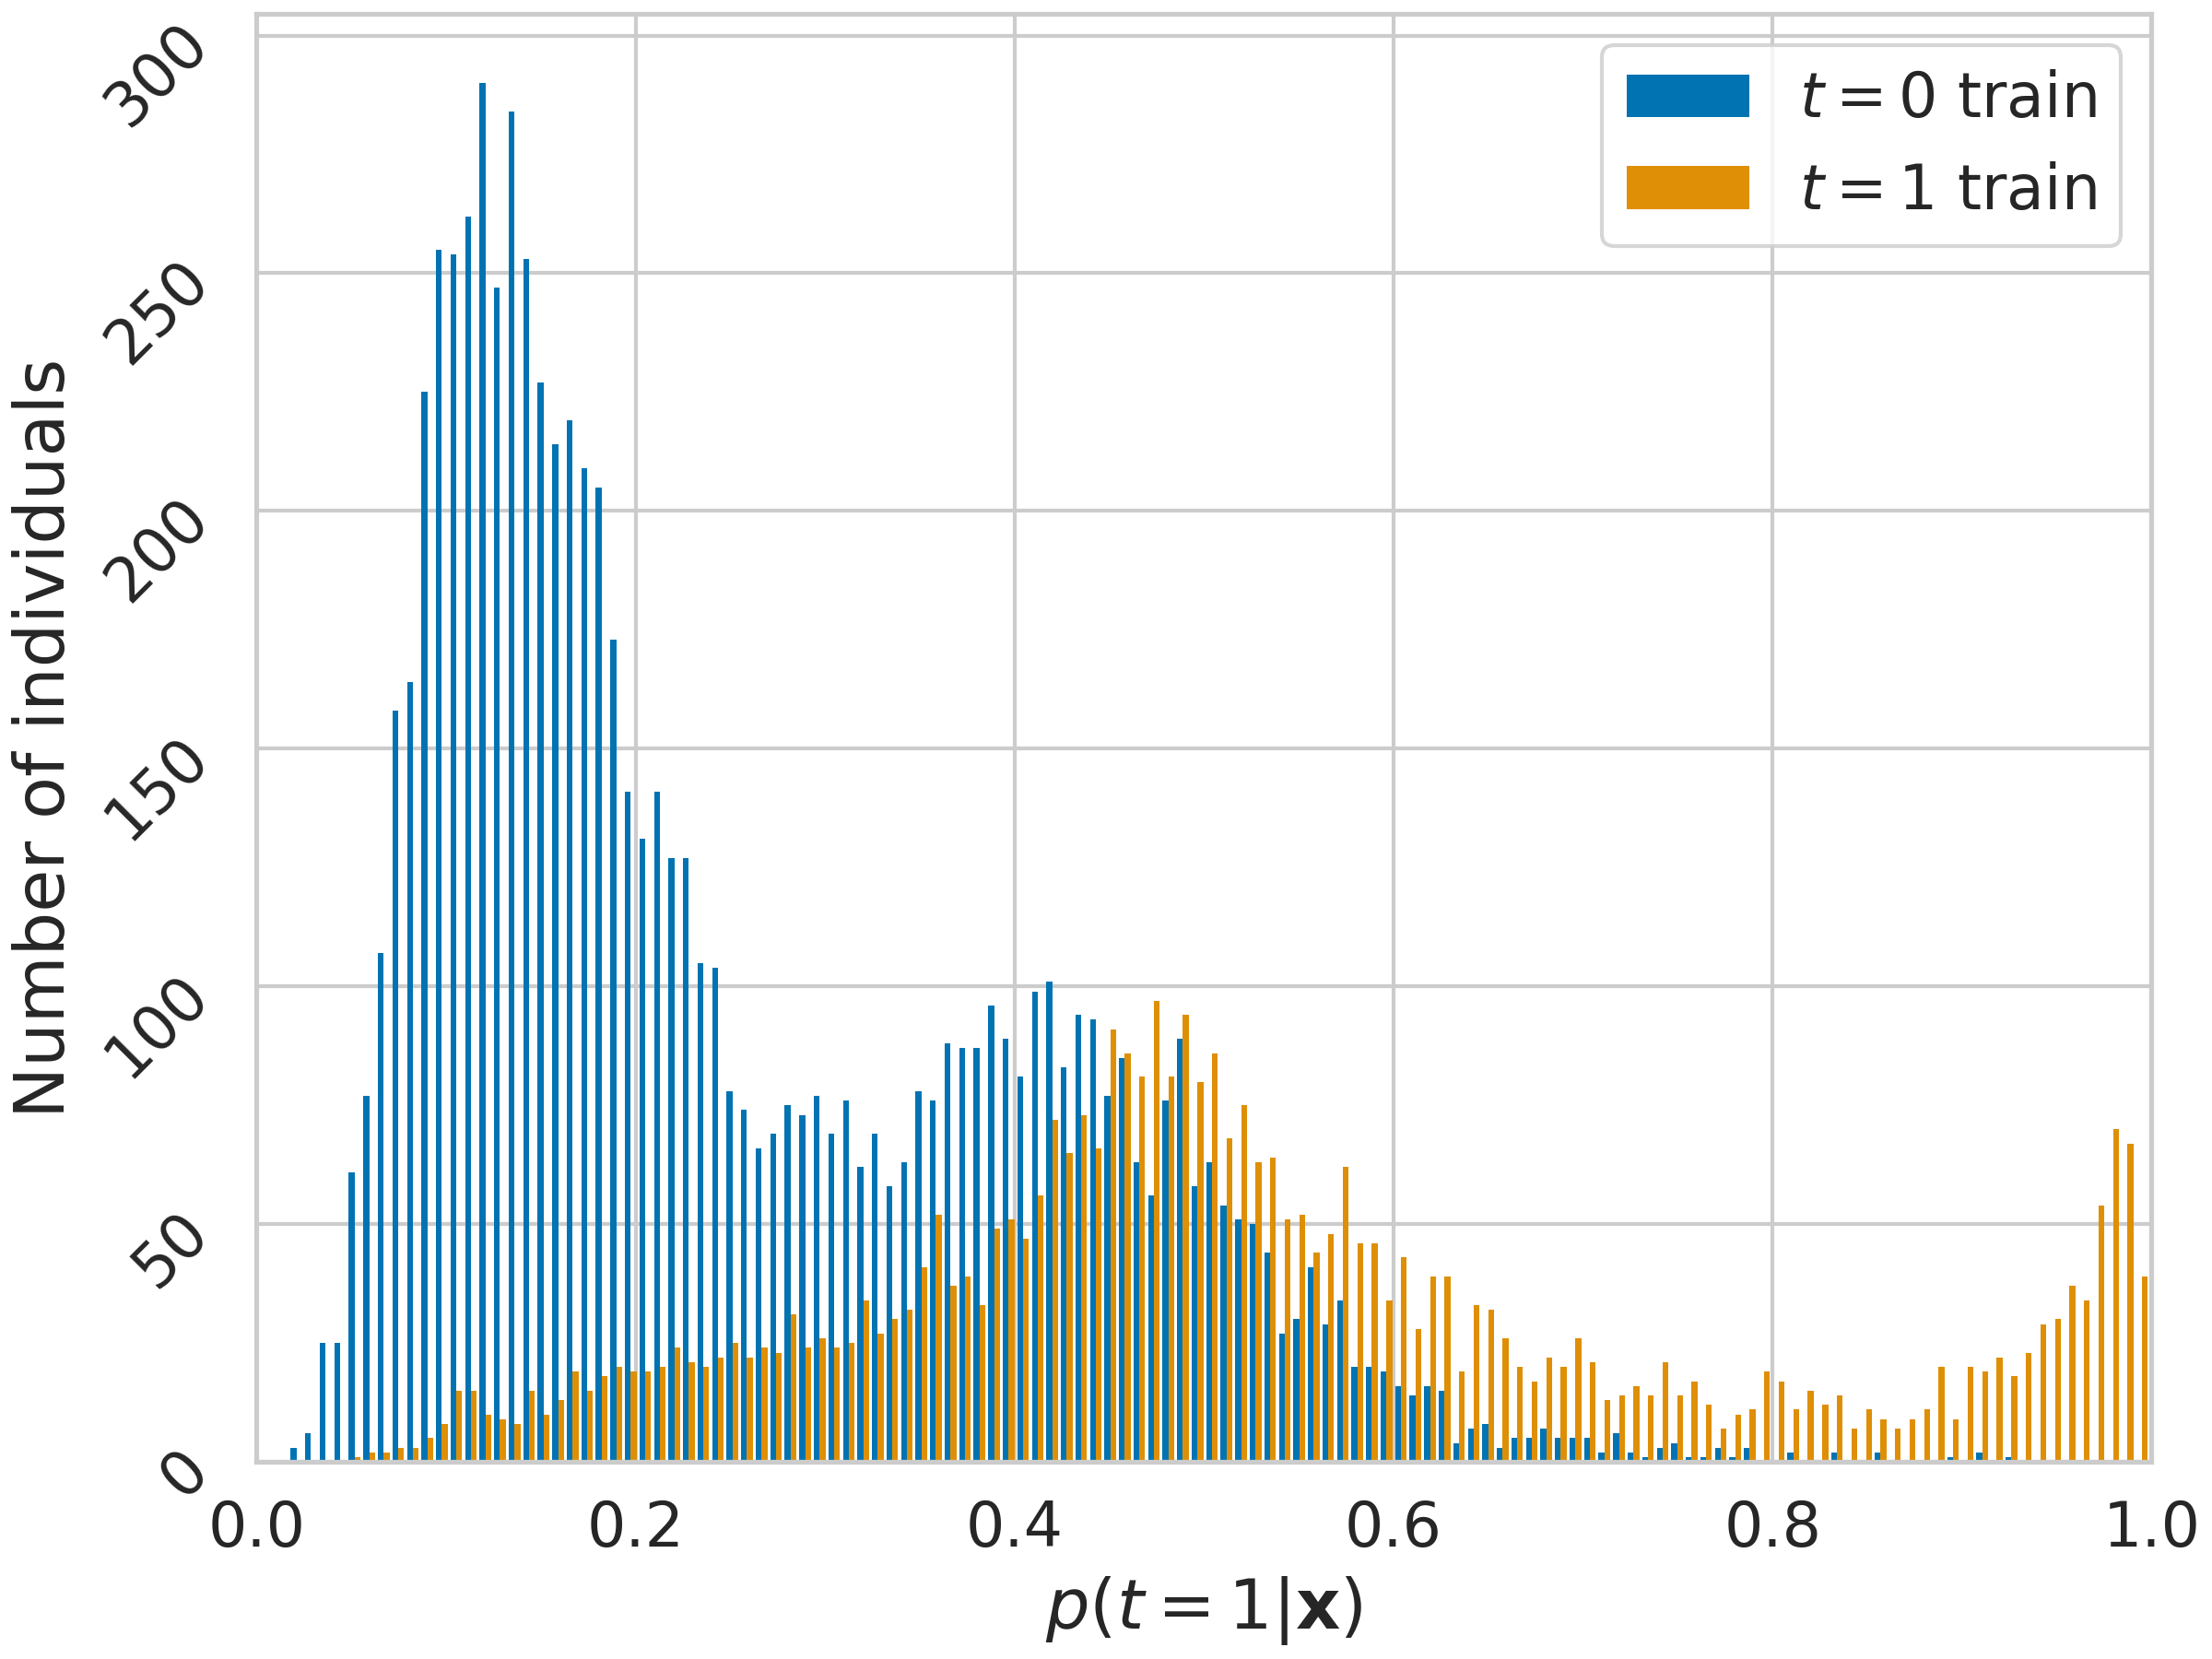
\includegraphics[width=\textwidth,height=0.52\textheight,keepaspectratio]{fig2a_cemnist_propensity.png}
\\\centering{\footnotesize Fig.\ 2a: propensity histogram. Peaks at left $=$ untreated nines.
Trimmer with $\eta{=}0.05$ removes nines, keeps twos.}
\end{columns}
\end{frame}

% -------------------------------------------------------
\begin{frame}{Core insight: non-overlap is covariate shift}

\textbf{Recall:} covariate shift = test distribution differs from training distribution.

\bigskip
Consider the model for the $T=1$ arm, trained on $p(X \mid T=1)$.

\begin{block}{Key reframing}
If $e(x) = \Prob(T=1 \mid x) \approx 0$, then by Bayes:
$p(x \mid T=1) \approx 0$.\\
So $x$ is \textbf{out-of-distribution} for the $T=1$ model.
\end{block}

\begin{itemize}
  \item $e(x)\approx 0$: $\mu_1(x)$ is OoD.
  \item $e(x)\approx 1$: $\mu_0(x)$ is OoD.
  \item Non-overlap $\Leftrightarrow$ at least one outcome model must extrapolate.
\end{itemize}

\bigskip
\begin{center}
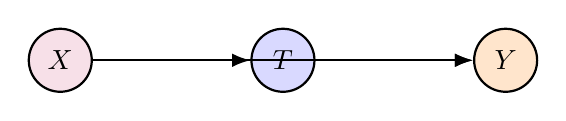
\begin{tikzpicture}[node distance=2cm]
  \node[conf]  (X) {$X$};
  \node[treat, right=of X] (T) {$T$};
  \node[outc,  right=of T] (Y) {$Y$};
  \draw[arrow] (X) -- (T);
  \draw[arrow] (X) -- (Y);
  \draw[arrow] (T) -- (Y);
\end{tikzpicture}\\[4pt]
\footnotesize Both $\mu_0$ and $\mu_1$ must be estimated; positivity ensures both have data.
\end{center}
\end{frame}

% -------------------------------------------------------
\begin{frame}{Epistemic vs.\ aleatoric uncertainty}

\begin{columns}
\column{0.46\textwidth}
\begin{block}{Aleatoric}
Inherent noise in $Y$.\\[4pt]
Cannot be reduced with more data.
\end{block}
\vspace{6pt}
\begin{block}{Epistemic}
Uncertainty from \emph{lack of data}.\\[4pt]
Disappears as more relevant data arrives.
\end{block}
\vspace{6pt}
We want to detect \textbf{epistemic} uncertainty in $\hat\tau(x)$.

\column{0.52\textwidth}
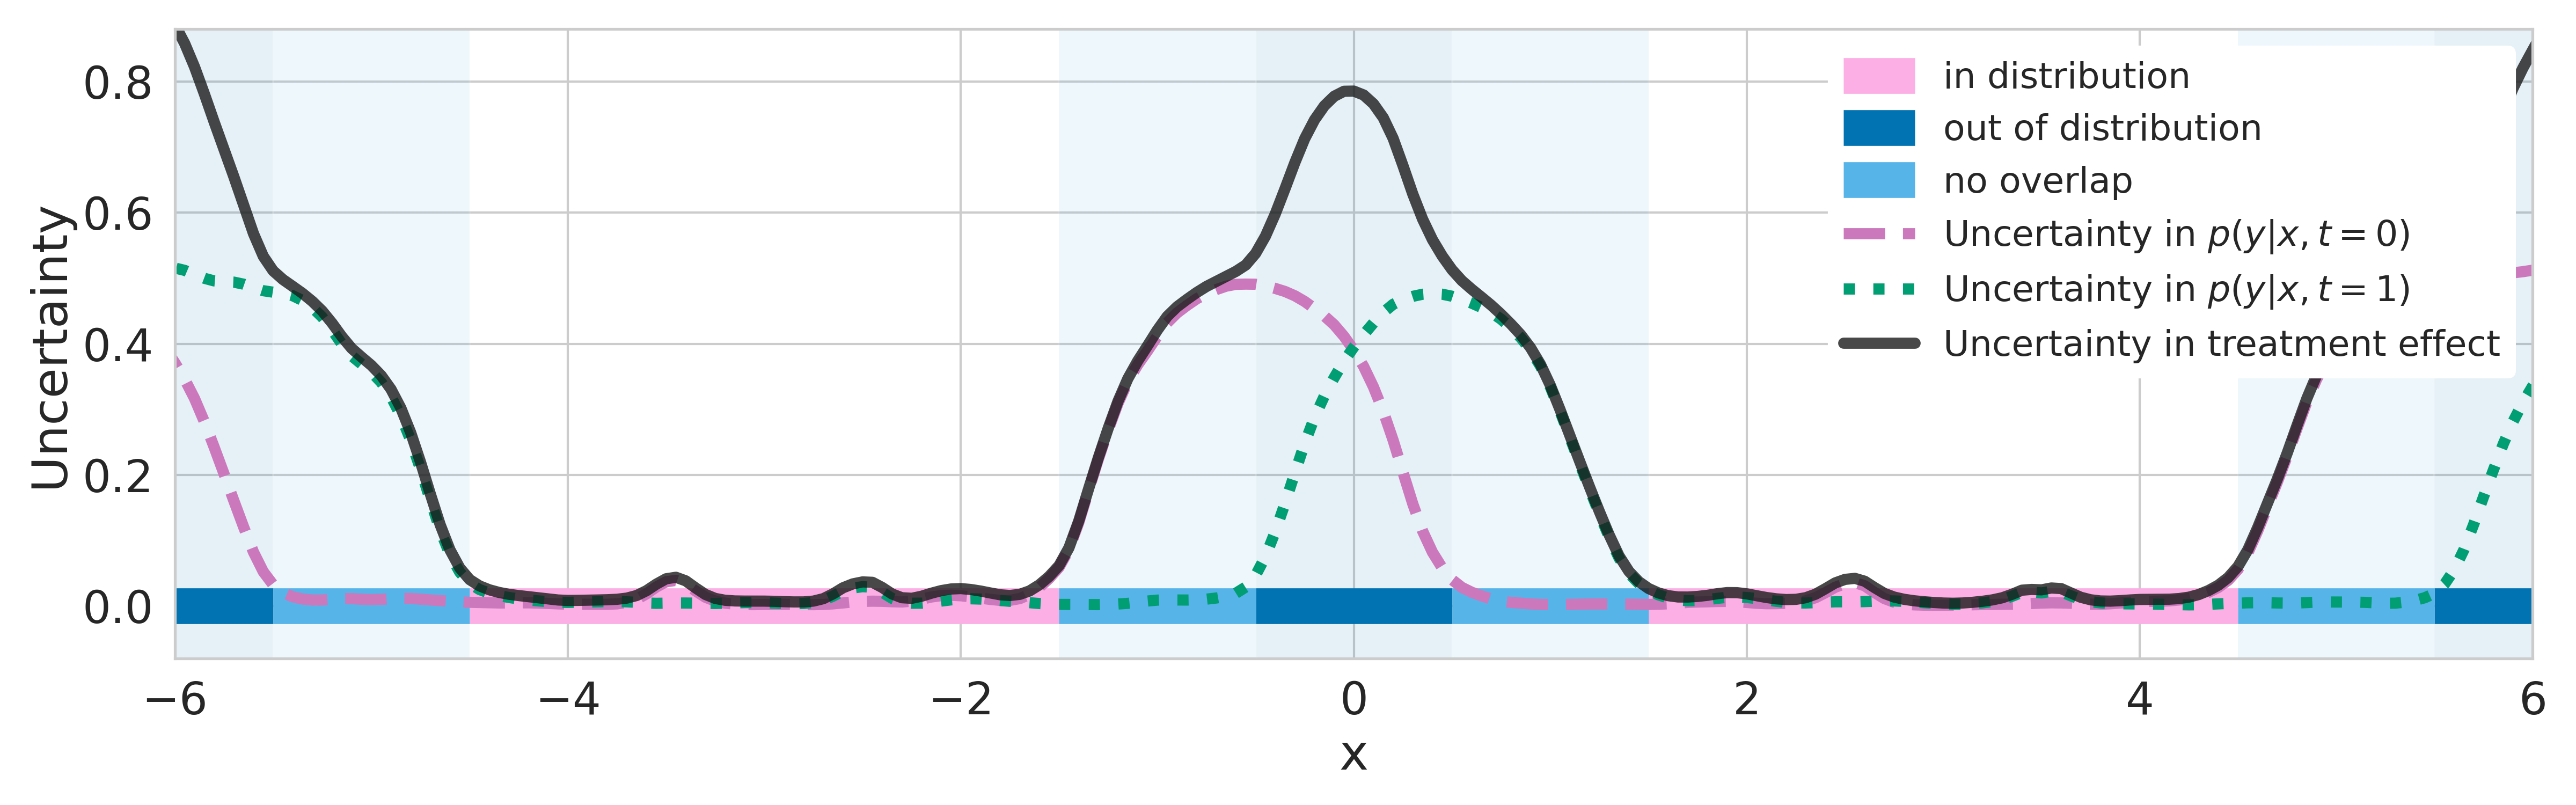
\includegraphics[width=\textwidth]{fig1c_cate_uncertainty.png}
\\\centering{\footnotesize Fig.\ 1 (bottom): CATE uncertainty is high where at least one arm model lacks data.}
\end{columns}
\end{frame}

% -------------------------------------------------------
\begin{frame}{Figure 1: BNN functions detect non-overlap}

\begin{columns}
\column{0.48\textwidth}
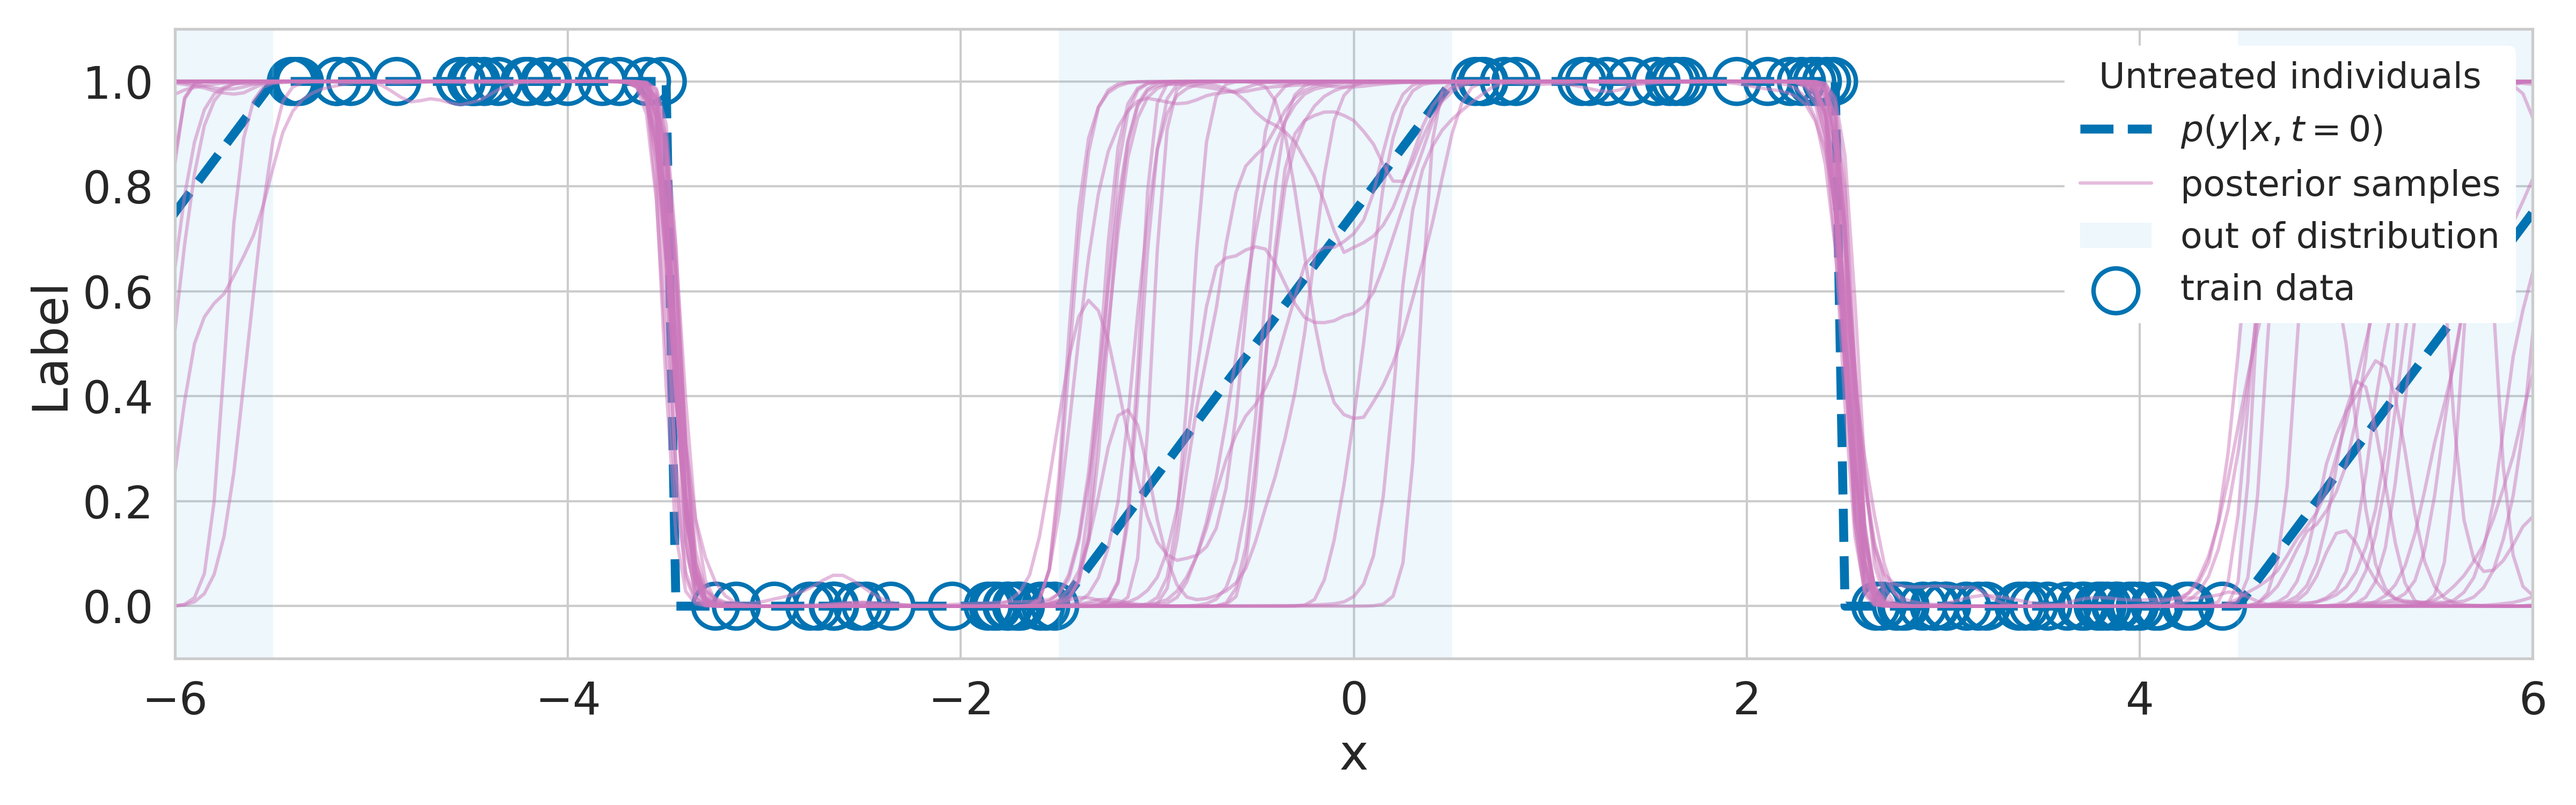
\includegraphics[width=\textwidth]{fig1a_bnn_t0.png}
\\\centering{\footnotesize $T=0$ arm: BNN functions agree in-distribution,\\
diverge where $p(x\mid T=0)\approx 0$ (right of shaded region).}

\column{0.48\textwidth}
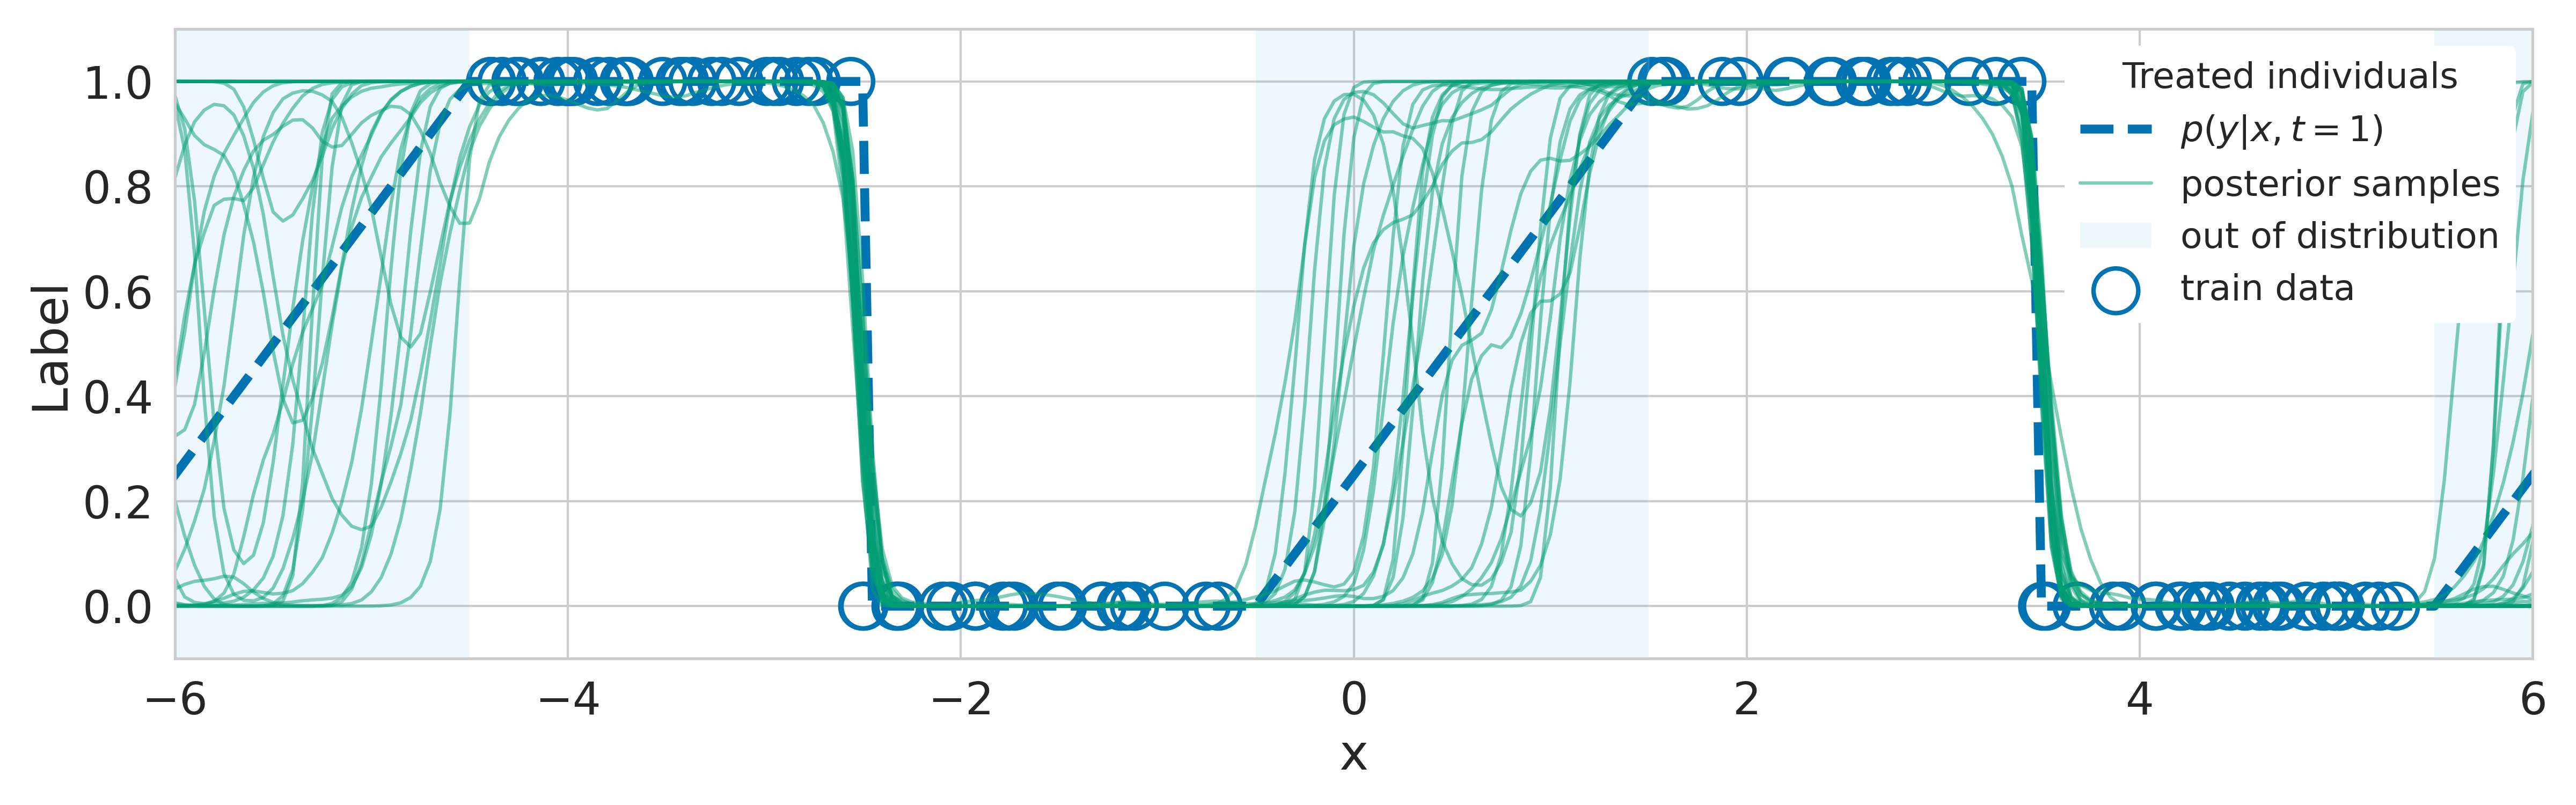
\includegraphics[width=\textwidth]{fig1b_bnn_t1.png}
\\\centering{\footnotesize $T=1$ arm: functions diverge where $p(x\mid T=1)\approx 0$\\
(left of shaded region = low-propensity units).}
\end{columns}

\bigskip
\begin{center}
\textit{High variance across BNN draws = epistemic uncertainty = model says ``I don't know.''}
\end{center}
\end{frame}

% -------------------------------------------------------
\begin{frame}{Bayesian neural networks: the tool}

Replace a single network $\mu_0(x;\,\omega_0)$ with a
\emph{distribution over networks}:
\[
p(\omega_0 \mid \mathcal{D}) \quad \text{(posterior over weights).}
\]

Epistemic uncertainty $\approx$ variance across sampled networks:
\[
U_0(x) = \mathrm{Var}_{\omega_0 \sim p(\omega_0\mid\mathcal{D})}
          \bigl[\mu_0(x;\,\omega_0)\bigr].
\]

\begin{block}{Practical approximation: MC Dropout (Gal \& Ghahramani, 2016)}
Add dropout to each outcome head.
Keep dropout \emph{on} at test time.
Each stochastic forward pass $\approx$ one draw from the approximate posterior.
\end{block}
\end{frame}

% -------------------------------------------------------
\begin{frame}{CATE uncertainty: the formal decomposition}

By the law of total variance:
\[
\mathrm{Var}\bigl[Y(1)-Y(0) \mid x\bigr]
=
\underbrace{
  \E_\omega\!\bigl[\mathrm{Var}_{Y}[\cdots]\bigr]
}_{\text{aleatoric}}
+
\underbrace{
  \mathrm{Var}_\omega\bigl[\mu_{\omega_1}(x) - \mu_{\omega_0}(x)\bigr]
}_{\text{epistemic in }\hat\tau(x)}
\]

The paper uses the epistemic term as its uncertainty signal:
\[
U(x) = \mathrm{Var}_\omega\bigl[\hat\tau(x)\bigr]
      = \mathrm{Var}_\omega\bigl[\mu_{\omega_1}(x) - \mu_{\omega_0}(x)\bigr].
\]

\begin{itemize}
  \item Estimated by sampling $\omega$ via MC Dropout at test time.
  \item $U(x)$ is large when at least one arm model is OoD at $x$.
  \item Captures both non-overlap \emph{and} input covariate shift.
\end{itemize}
\end{frame}

% -------------------------------------------------------
\begin{frame}{Neural CATE estimators: a brief map}

\begin{center}
\small
\renewcommand{\arraystretch}{1.3}
\begin{tabular}{lll}
\toprule
Model      & Key idea                                      & Bayesian extension \\
\midrule
T-Learner  & Fit $\mu_0$, $\mu_1$ separately               & B-TLearner \\
TARNet     & Shared representation, separate outcome heads & BTARNet \\
CFRNet     & TARNet $+$ MMD regularisation for overlap     & BCFR-MMD \\
Dragonnet  & TARNet $+$ joint propensity prediction        & BDragonnet \\
CEVAE      & Latent confounders via VAE                    & BCEVAE $+$ neg.\ sampling \\
\bottomrule
\end{tabular}
\end{center}

\bigskip
\textbf{Paper's recipe:} add MC Dropout to the outcome heads of any model
$\Rightarrow$ get $U(x)$ for free, with minimal code changes.
\end{frame}

% -------------------------------------------------------
\begin{frame}{Rejection policy: thresholding on uncertainty}

\textbf{Decision rule:} given rejection budget $r_{\mathrm{rej}}$,
withhold recommendation for the $r_{\mathrm{rej}}$ fraction with highest $U(x)$.

\bigskip
\begin{columns}
\column{0.46\textwidth}
\textbf{Uncertainty policy}
\[
\text{reject } x \;\text{ if }\; U(x) > \kappa
\]
Detects non-overlap and covariate shift.

\column{0.46\textwidth}
\textbf{Propensity trimming}
\[
\text{reject } x \;\text{ if }\; \hat{e}(x) < \eta \;\text{ or }\; > 1{-}\eta
\]
Captures marginal probability only.\\
Trims nines, keeps twos (CEMNIST).
\end{columns}

\bigskip
\textbf{Metric:} recommendation error rate and $\sqrt{\mathrm{PEHE}}$
on the non-rejected subset, at fixed $r_{\mathrm{rej}}$.
\end{frame}

% -------------------------------------------------------
\begin{frame}{Results: CEMNIST --- uncertainty beats propensity}

\begin{center}
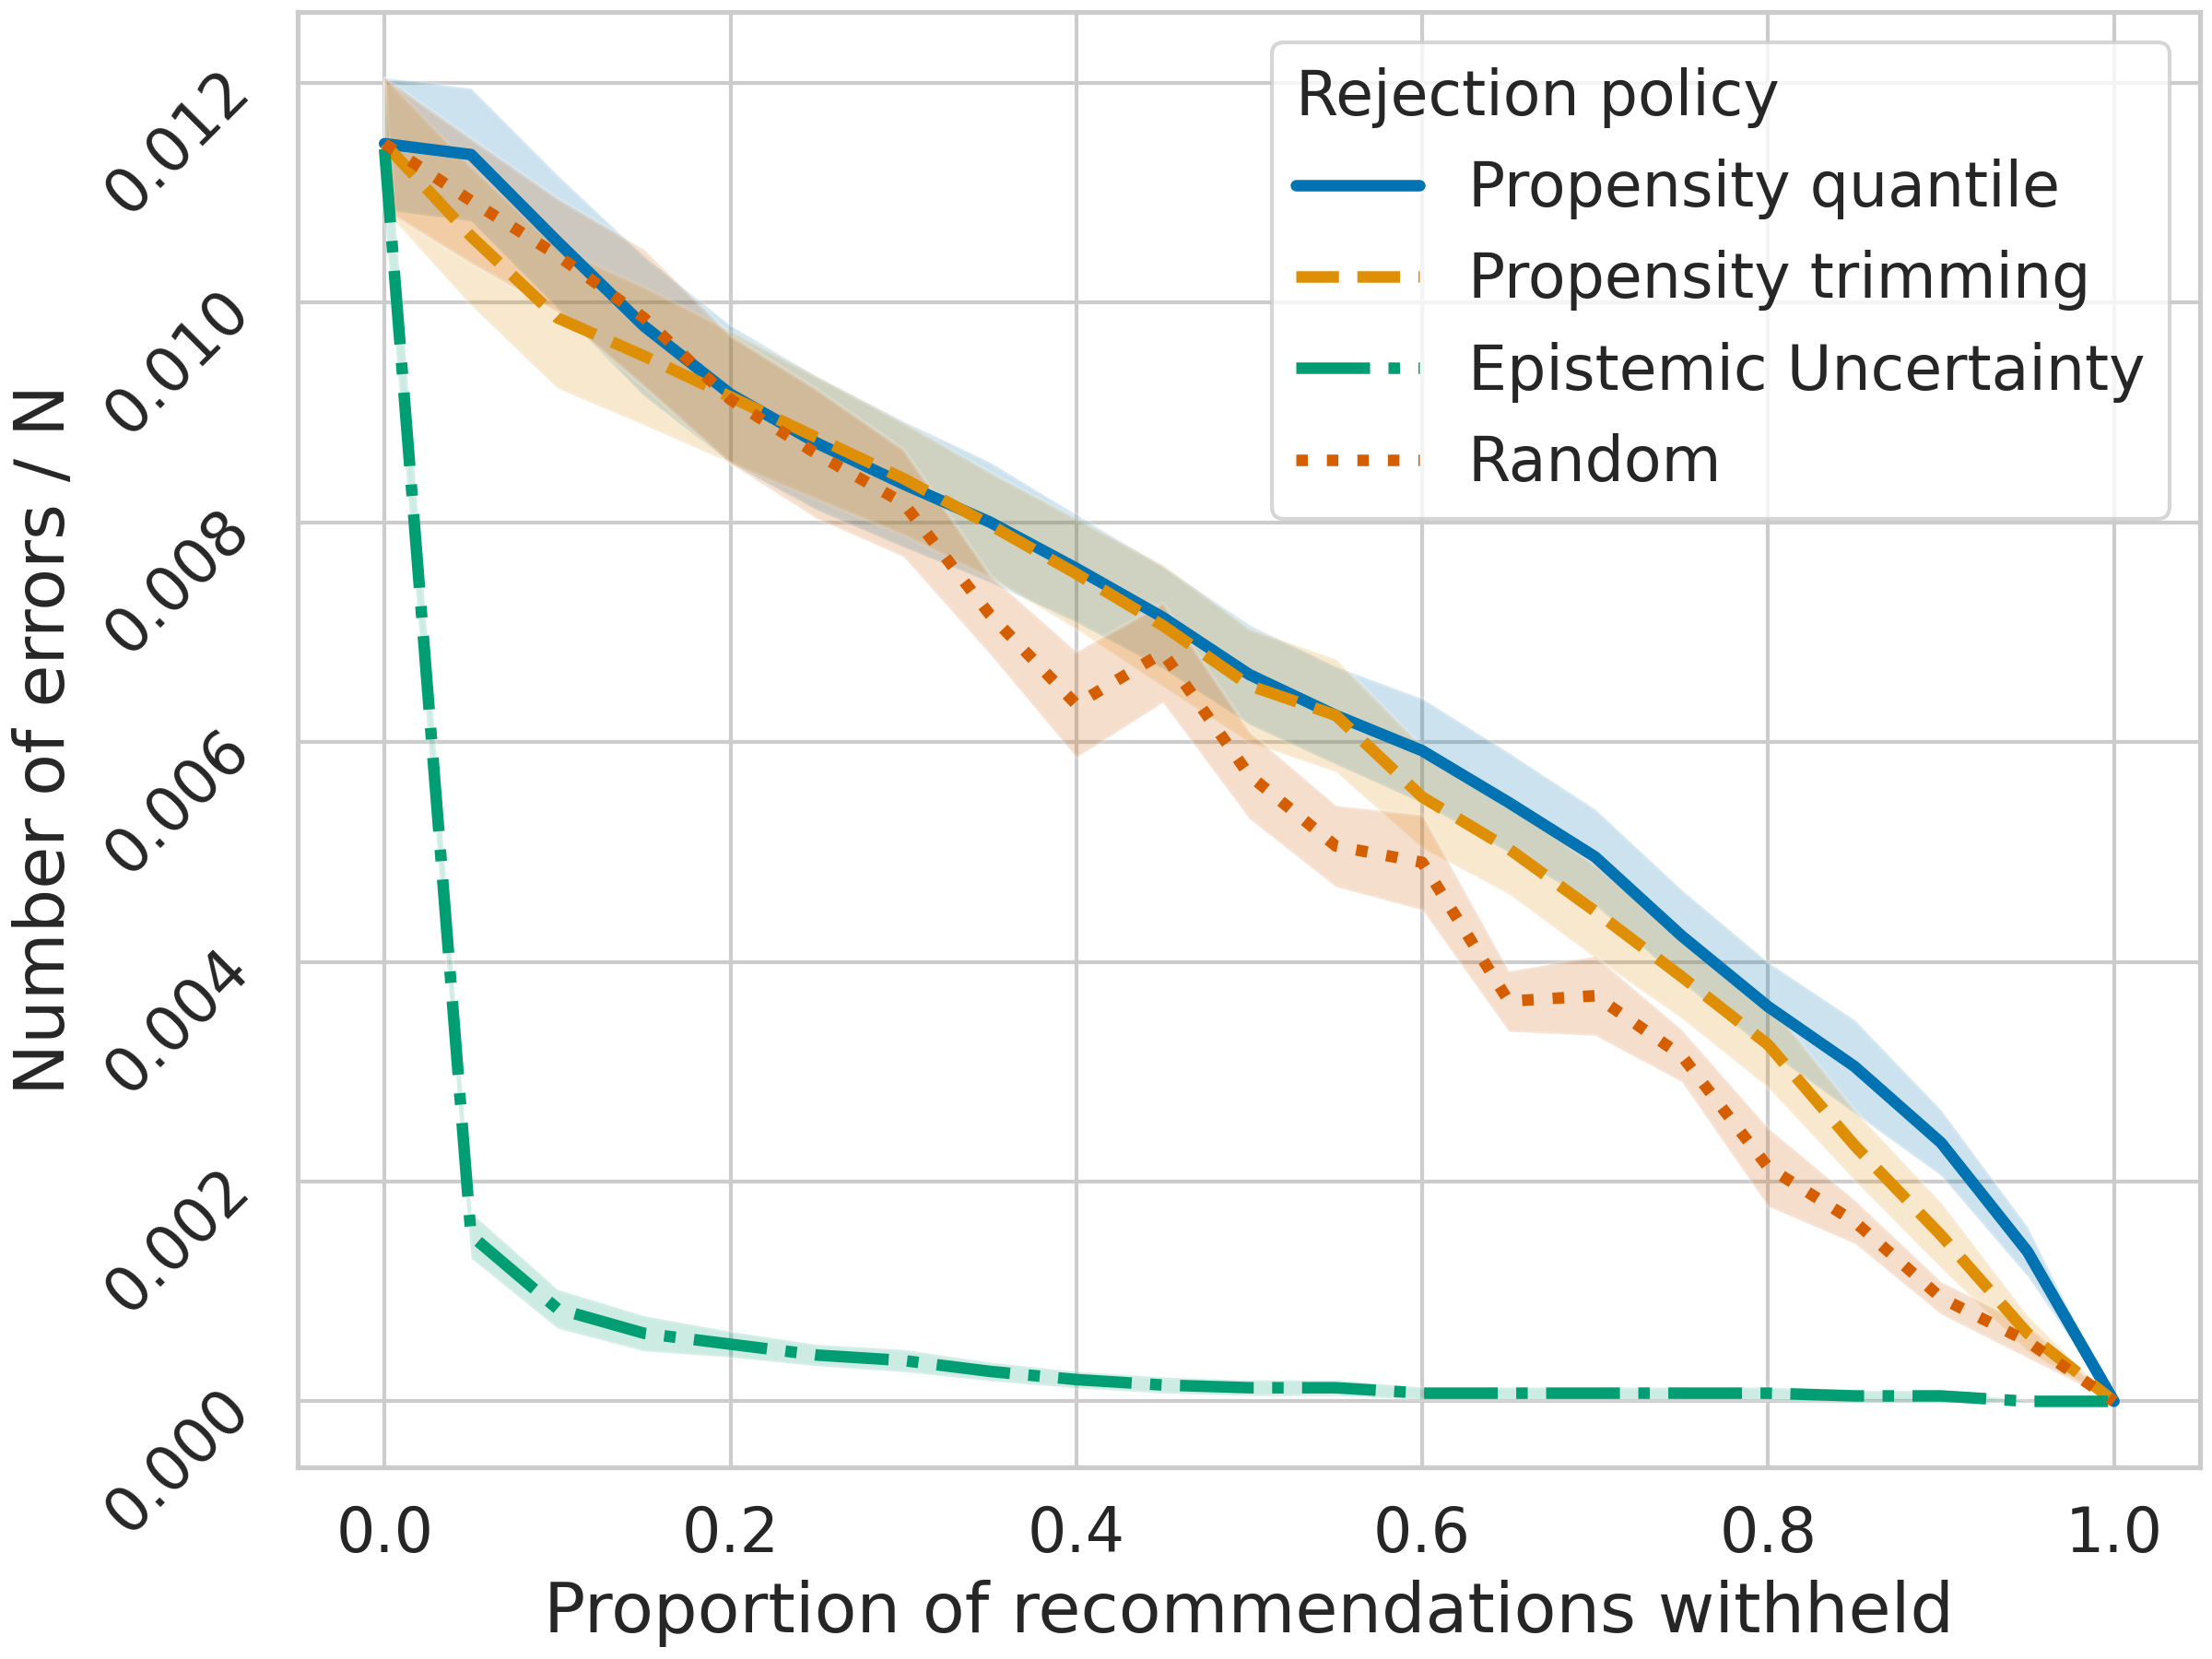
\includegraphics[width=0.68\textwidth,height=0.62\textheight,keepaspectratio]{fig2b_cemnist_errorrate.png}
\\[2pt]
{\footnotesize Fig.\ 2b: error rate vs.\ rejection rate on CEMNIST.
\textbf{Green} (uncertainty) $\ll$ orange/blue (propensity) across the full range.}
\end{center}
\end{frame}

% -------------------------------------------------------
\begin{frame}{Results: IHDP and ACIC 2016}

\begin{columns}
\column{0.60\textwidth}
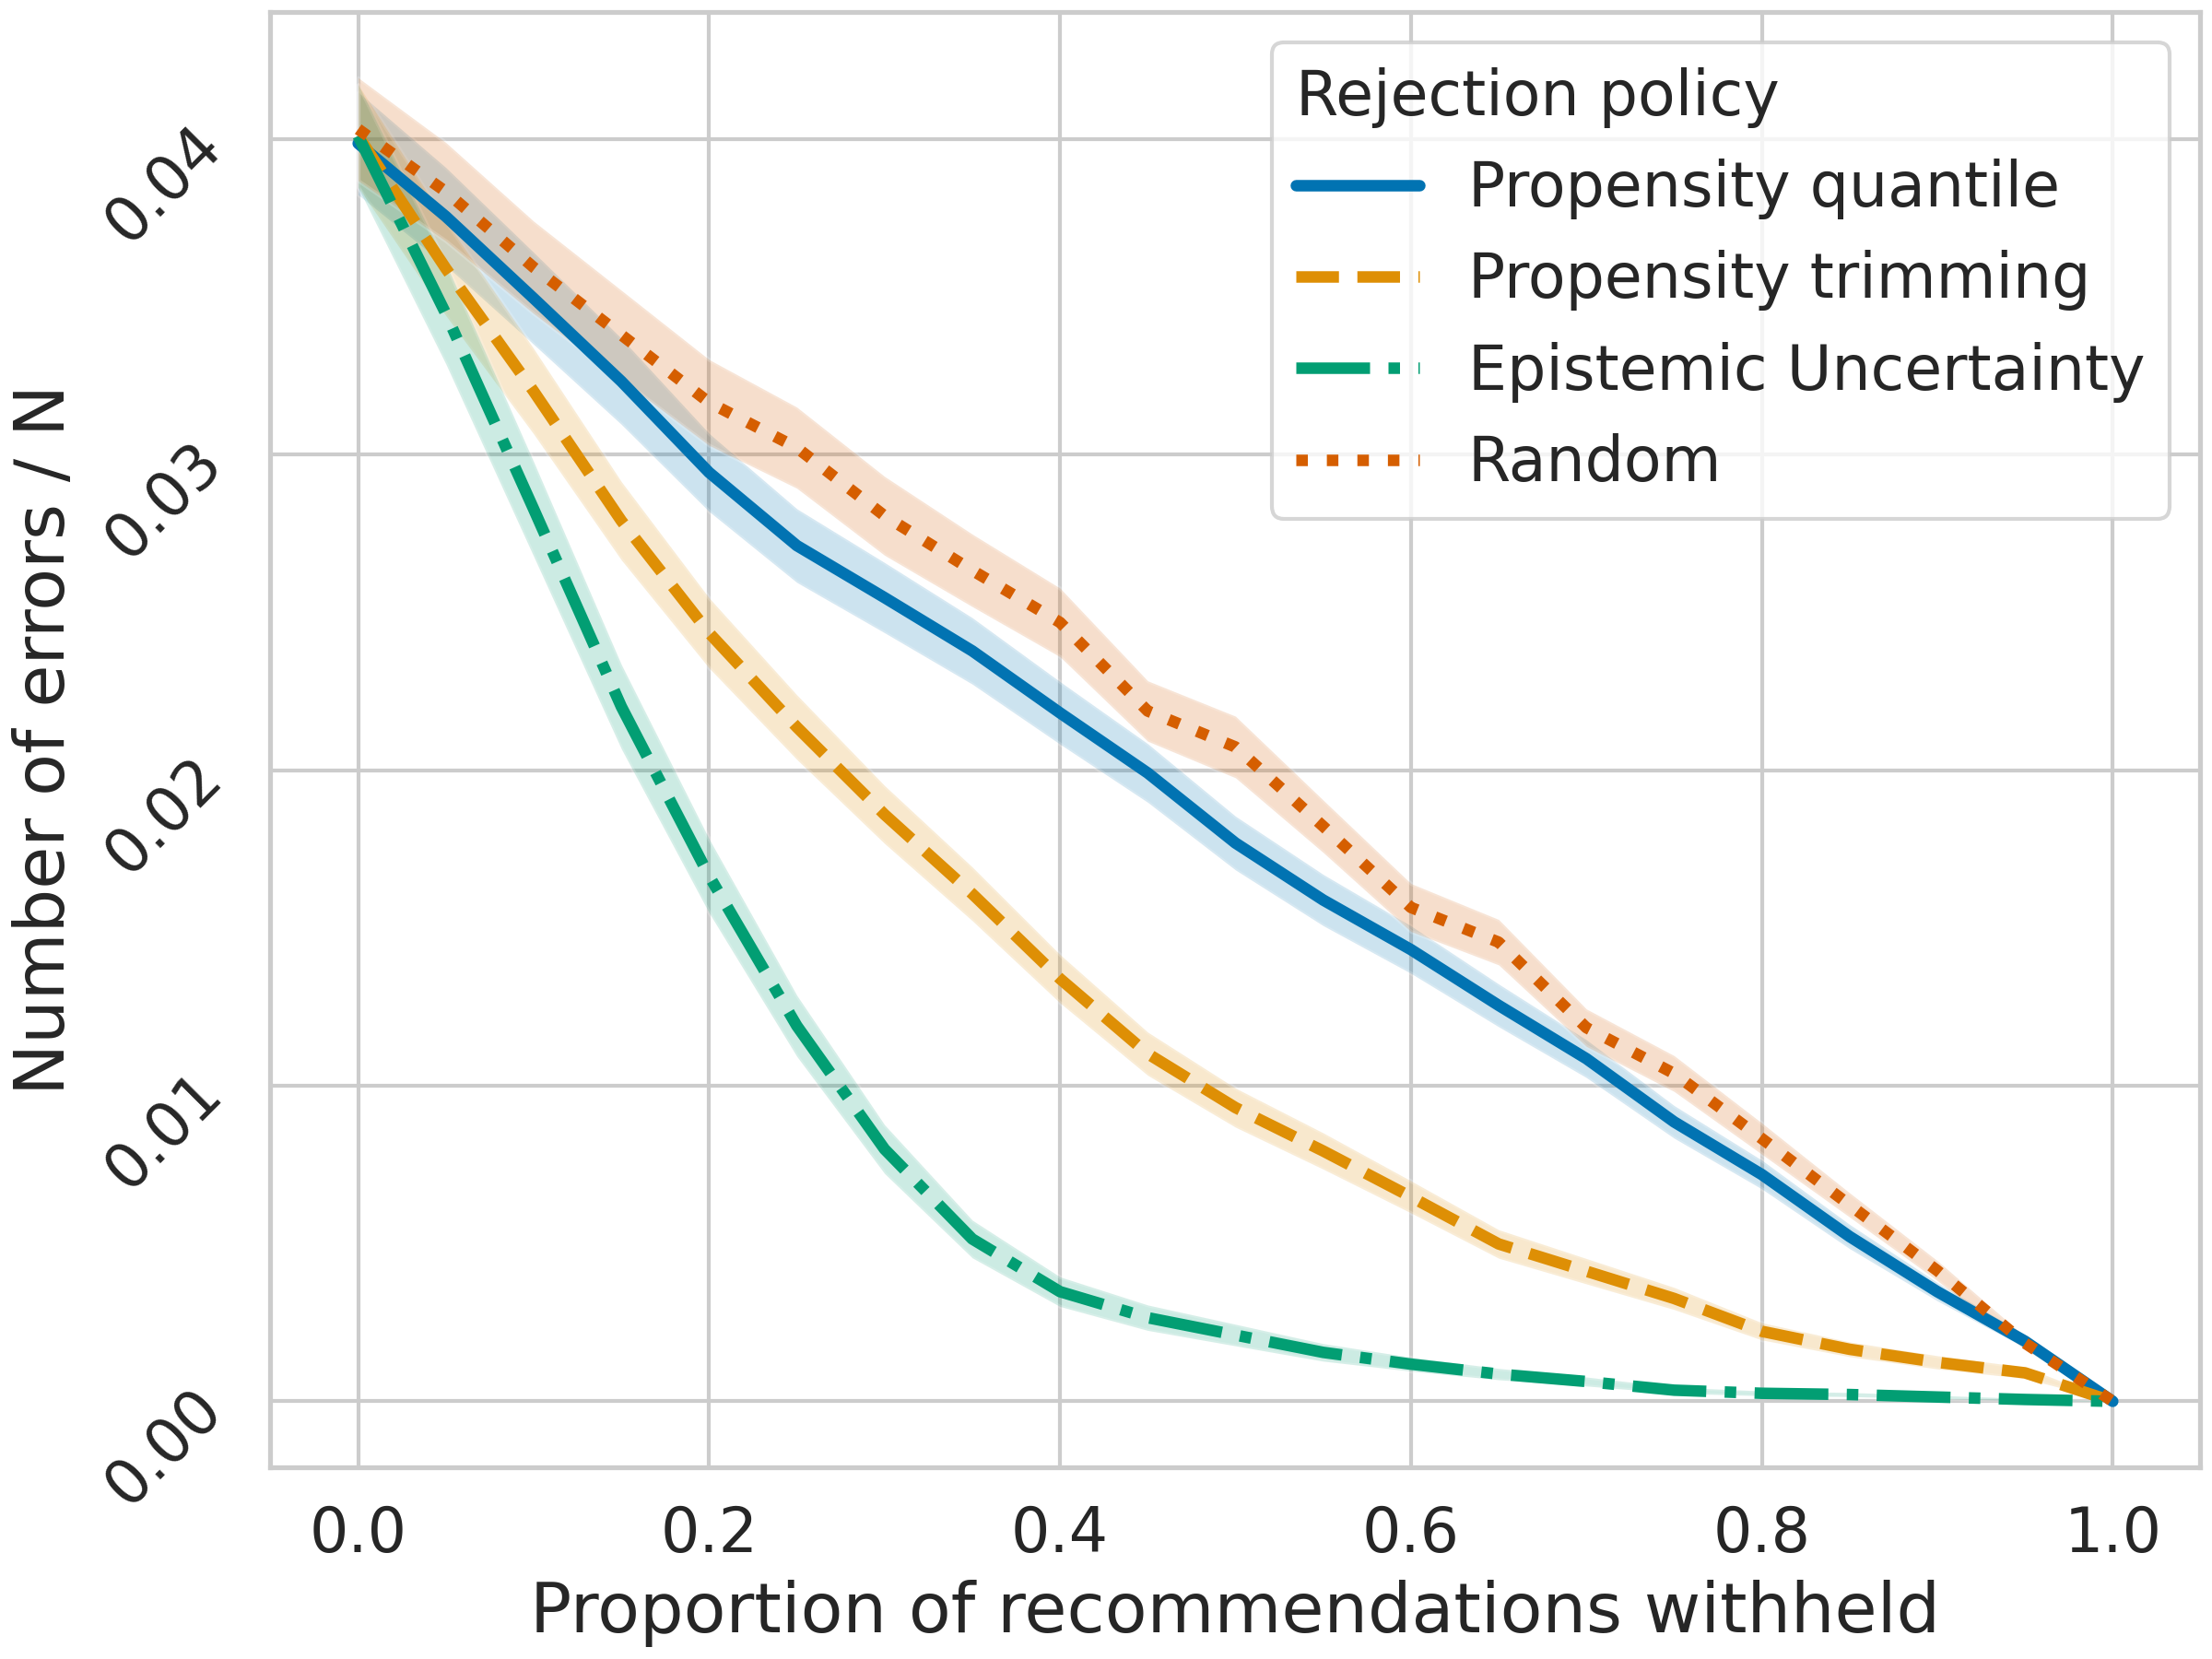
\includegraphics[width=\textwidth,height=0.58\textheight,keepaspectratio]{fig3b_ihdp_covshift.png}
\\\centering{\footnotesize Fig.\ 3b: IHDP Covariate Shift.
Uncertainty (green) outperforms propensity across all rejection rates.}

\column{0.38\textwidth}
\small
Same result on:
\begin{itemize}
  \item IHDP (no shift)
  \item ACIC 2016
\end{itemize}
\medskip
All model classes improve.\\[4pt]
Uncertainty is \textbf{more data-efficient}: lower error at the same rejection rate.
\end{columns}
\end{frame}

% -------------------------------------------------------
\begin{frame}{Part 1 recap}

\begin{block}{What Jesson et al.\ (2020) show}
\begin{enumerate}
  \item Non-overlap $=$ covariate shift for one outcome model.
  \item Epistemic uncertainty in BNNs detects this, and detects
        input covariate shift as a bonus.
  \item MC Dropout is a cheap, practical approximation.
  \item Uncertainty-based rejection outperforms propensity trimming,
        especially when $e(x)$ and CATE estimability are decorrelated.
\end{enumerate}
\end{block}

\bigskip
\begin{center}
\Large\textit{Now: how much should we trust this?}
\end{center}
\end{frame}

% =======================================================
\section{Part 2: Critical Evaluation}
% =======================================================

% -------------------------------------------------------
\begin{frame}{Assumption audit}

\begin{center}
\renewcommand{\arraystretch}{1.3}
\small
\begin{tabular}{p{5.5cm}p{2.8cm}p{3.5cm}}
\toprule
Assumption & Paper status & Notes \\
\midrule
Unconfoundedness:\\
$(Y(1),Y(0))\indep T\mid X$
  & \alert{Assumed, untested}
  & Foundation of all CATE claims \\
SUTVA / consistency
  & \alert{Assumed, untested}
  & Standard in literature \\
Positivity $0 < e(x) < 1$
  & \textcolor{green!60!black}{Relaxed}
  & The paper's contribution \\
Correct model class
  & \alert{Assumed}
  & NN may misspecify $\mu_t$ \\
i.i.d.\ training data
  & \alert{Assumed}
  & Violated under deployment shift \\
\bottomrule
\end{tabular}
\end{center}

\bigskip
\begin{alertblock}{}
The paper relaxes positivity. It inherits all other classical assumptions intact.
\end{alertblock}
\end{frame}

% -------------------------------------------------------
\begin{frame}{The unconfoundedness blindspot}

The method tells you \textbf{when the model is uncertain}.
It does not tell you \textbf{whether the model is biased}.

\bigskip
If unconfoundedness fails --- a hidden $U$ confounds both $T$ and $Y$:

\begin{center}
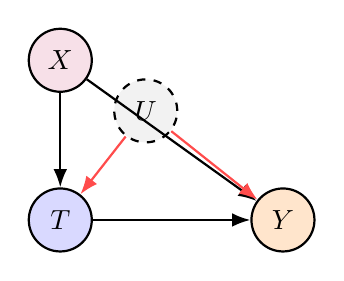
\begin{tikzpicture}[node distance=2cm]
  \node[treat] (T) {$T$};
  \node[outc, right=of T] (Y) {$Y$};
  \node[conf, above=1.2cm of T] (X) {$X$};
  \node[hidden, above right=0.8cm and 0.5cm of T] (U) {$U$};
  \draw[arrow] (T) -- (Y);
  \draw[arrow] (X) -- (T);
  \draw[arrow] (X) -- (Y);
  \draw[badpath] (U) -- (T);
  \draw[badpath] (U) -- (Y);
\end{tikzpicture}
\end{center}

\begin{itemize}
  \item $\hat\mu_1(x)$ and $\hat\mu_0(x)$ both absorb the confounding signal.
  \item \alert{$U(x) = \mathrm{Var}_\omega[\hat\tau(x)]$ can be small even when bias is large.}
\end{itemize}

\begin{block}{}
A Bayesian causal model can be \emph{confidently wrong} under hidden confounding.
\end{block}
\end{frame}

% -------------------------------------------------------
\begin{frame}{Two failure modes: only one is addressed}

\begin{center}
\renewcommand{\arraystretch}{1.8}
\begin{tabular}{r|p{4.6cm}p{4.6cm}}
 & \textbf{Low bias} & \textbf{High bias (hidden confounding)} \\
\hline
\textbf{High $U(x)$}
  & \textcolor{green!60!black}{Reject $\Rightarrow$ safe.}
  & \textcolor{green!60!black}{Reject $\Rightarrow$ safe (by luck).} \\
\hline
\textbf{Low $U(x)$}
  & \textcolor{green!60!black}{Recommend $\Rightarrow$ safe.}
  & \alert{Recommend $\Rightarrow$ confidently wrong.}
    \textbf{Blind spot.} \\
\end{tabular}
\end{center}

\bigskip
The paper operates in the left column and top row.\\
The bottom-right cell is untouched.
\end{frame}

% -------------------------------------------------------
\begin{frame}{What about sensitivity analysis?}

Classical tools address hidden confounding directly:

\begin{itemize}
  \item \textbf{Rosenbaum bounds:} how large must hidden $U$ be to
        overturn the conclusion?
  \item \textbf{E-values:} minimum confounder strength to explain away the effect.
  \item \textbf{Random common cause refuters} (DoWhy): add a synthetic
        unobserved confounder; check if the estimate changes.
\end{itemize}

\bigskip
\begin{alertblock}{The paper has no sensitivity analysis.}
It tells us \emph{when} to trust a CATE estimate (overlap, in-distribution).
It does not tell us \emph{how robust} the estimate is to hidden confounding.
\end{alertblock}

\bigskip
Uncertainty quantification and sensitivity analysis are \textbf{orthogonal}.
A complete pipeline needs both.
\end{frame}

% -------------------------------------------------------
\begin{frame}{The benchmarking problem}

All experiments use \textbf{semi-synthetic} datasets:

\begin{itemize}
  \item \textbf{IHDP}: real covariates from a clinical trial; synthetic outcomes.
  \item \textbf{ACIC 2016}: synthetic competition data; known ground truth.
  \item \textbf{CEMNIST}: MNIST digits; synthetic treatment and outcomes.
\end{itemize}

\bigskip
In semi-synthetic data, true CATE is known by construction
$\Rightarrow$ $\sqrt{\mathrm{PEHE}}$ is computable.

\bigskip
\begin{alertblock}{In real-world observational data}
$Y_i(0)$ for treated units is \textbf{never observed}.\\
$\sqrt{\mathrm{PEHE}}$ is \textbf{uncomputable}.\\
The paper's main metric cannot be verified in deployment.
\end{alertblock}
\end{frame}

% -------------------------------------------------------
\begin{frame}{Comparison to classical methods}

\begin{center}
\small
\renewcommand{\arraystretch}{1.4}
\begin{tabular}{p{3.5cm}p{4cm}p{4cm}}
\toprule
 & \textbf{Propensity trimming} & \textbf{Uncertainty rejection} \\
\midrule
Detects non-overlap & Yes, via $\hat e(x)$ & Yes, more precisely \\
Handles covariate shift & No & Yes \\
Handles hidden confounding & No & No \\
Sensitivity analysis & Rosenbaum / E-values & None \\
Computationally cheap & Yes & No (BNN training) \\
Principled threshold & Caliendo \& Kopeinig & No principled rule \\
Verifiable on real data & Yes & Yes, but $\sqrt{\mathrm{PEHE}}$ uncomputable \\
\bottomrule
\end{tabular}
\end{center}
\end{frame}

% -------------------------------------------------------
\begin{frame}{What the paper genuinely contributes}

\begin{enumerate}
  \item \textbf{Elegant reframing.}
        Non-overlap $=$ covariate shift for one arm.
        Opens a toolkit (BNNs, OoD detection) not previously applied here.

  \item \textbf{Practical method.}
        MC Dropout adds uncertainty to any neural causal model
        with minimal engineering cost.

  \item \textbf{New benchmark.}
        CEMNIST exposes a concrete failure mode of propensity trimming
        in high-dimensional, reproducible settings.

  \item \textbf{Better rejection.}
        Outperforms propensity trimming on IHDP, ACIC, and CEMNIST
        across five model architectures.
\end{enumerate}

\bigskip
\begin{block}{What it does not contribute}
A solution to hidden confounding, a sensitivity analysis, or a way to
validate CATE estimates where ground truth is unavailable.
\end{block}
\end{frame}

% -------------------------------------------------------
\begin{frame}{Discussion questions --- Part A}

\begin{enumerate}

  \item \textbf{Uncertainty and confounding.}
        The paper assumes unconfoundedness throughout.
        If there are hidden confounders, can high $U(x)$ protect you?
        What would need to change to also catch confounding bias?

  \bigskip
  \item \textbf{Real-world validation.}
        The results are on semi-synthetic data.
        What experiment --- using only observational data without known CATE ---
        would convince you this holds in clinical practice?

  \bigskip
  \item \textbf{Redundancy with CFRNet.}
        CFRNet already penalises for overlap via MMD regularisation.
        Does MC Dropout on top give something genuinely new,
        or is it partially redundant?

\end{enumerate}
\end{frame}

% -------------------------------------------------------
\begin{frame}{Discussion questions --- Part B}

\begin{enumerate}
  \setcounter{enumi}{3}

  \item \textbf{What has the model contributed?}
        You run the method and get high $U(x)$ for a patient.
        You withhold the recommendation and defer to a clinician.
        What has the causal model actually contributed?
        Is detecting uncertainty enough?

  \bigskip
  \item \textbf{Uncertainty about what, exactly?}
        The paper estimates $U(x) = \mathrm{Var}_\omega[\hat\tau(x)]$.
        Is this the same as uncertainty about the true causal effect $Y(1)-Y(0)$?
        What components of total uncertainty are missing?

\end{enumerate}
\end{frame}

% -------------------------------------------------------
\begin{frame}{Take-away}

\[
U(x) = \mathrm{Var}_\omega\bigl[\hat\mu_{\omega_1}(x) - \hat\mu_{\omega_0}(x)\bigr]
\]

\begin{itemize}
  \item \textbf{What the paper gives you:}
        a principled signal for when to withhold a CATE estimate ---
        detecting non-overlap and covariate shift simultaneously.

  \item \textbf{What it assumes and does not question:}
        unconfoundedness, correct model class, i.i.d.\ data.
        High $U(x)$ is not a guard against confounding bias.
\end{itemize}

\bigskip
\begin{block}{The deeper lesson}
\textbf{Identification and uncertainty quantification are orthogonal.}\\
You can know exactly how uncertain you are about the wrong estimand.\\
Epistemic uncertainty $\neq$ robustness to assumption violations.
\end{block}
\end{frame}

\end{document}
